\section{Frequenzanalyse}
\subsection{Fourier-Transformation}
\script{121} Um vom Zeitbereich in Frequenzbereich zu Transformieren mitt Funktion $f(t)$ mit der Fourier-Transformation integriert werden:
\[
	F(j\omega) = \int_{-\infty}^{\infty}f(t)e^{-j\omega t}dt
\]

Die Rücktransformation mit der inverse Fourier-Transformation:
\[
f(t) = \frac{1}{2\pi}\int_{-\infty}^{\infty}F(j\omega)e^{j\omega t}d\omega
\]

Die Konvergenzgeschwindigkeit kann im \script{123} nachgelesen werden.

\subsubsection{Eigenschaften}
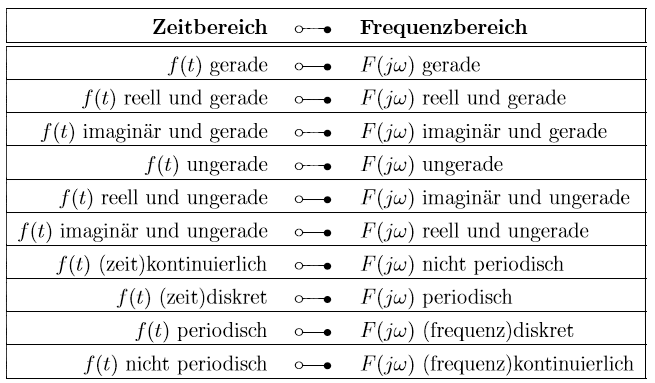
\includegraphics[width=\columnwidth]{Images/fourier_eigenschaten}
Weitere Eigenschaften sind im Skript auf Seite \script{124} zufinden.

\subsubsection{Symmetrie}
\textbf{ACHTUNG:} Gilt nur für $\mathbb{R}$ Fourierreihe! In $\mathbb{C}$ Reihe darf nicht über die halbe Periode Integriert und das Resultat verdoppelt werden! 
~\\
~\\
\noindent Für alle \textbf{geraden} (Achsensymmetrisch) T-periodische Funktionen ($f(t) = f(-t)$)  gilt $b_n = 0$ und für $a_n$ gilt:
\[
a_n = \frac{4}{T}\int_{0}^{\frac{T}{2}}f(t) \cdot \cos(n\omega t)dt
\]

\noindent Ist die Funktion \textbf{ungerade} (Punktsymmetrisch) ($f(-t) = -f(t)$) dann gilt $a_n = 0$ und für $b_n$:
\[
b_n = \frac{4}{T}\int_{0}^{\frac{T}{2}}f(t) \cdot \sin(n\omega t)dt 
\]


\subsubsection{Eigenschaften}
Einige wichtige Eigenschaften, weitere sind im \script{24}\\
\noindent\textbf{Funktionen}
\begin{align*}
	\delta(t) &\transform 1(\omega) \\
	u(t) &\transform \frac{1}{j\omega} \quad\text{(Einheitssprung)}\\
	\text{rect}_{-\frac{1}{2},\frac{1}{2}}(t) &\transform \sinc\left(\frac{\omega}{2}\right) \\
	\cos(\omega_0 t) &\transform \pi\left[\delta(\omega + \omega_0) + \delta(\omega - \omega_0)\right] \\
	\sin(\omega_0 t) &\transform j\pi\left[\delta(\omega + \omega_0) - \delta(\omega - \omega_0)\right]
\end{align*}

\noindent\textbf{Vertauschung}
\begin{align*}
	X(t) \transform 2\pi \cdot x(\-\omega)
\end{align*}

\noindent\textbf{Verschiebung im Zeitbereich}
\begin{align*}
	x(t - t_0) \transform X(\omega) \cdot e^{-j\omega t_0} 
\end{align*}

\noindent\textbf{Verschiebung im Frequenzbereich}
\begin{align*}
	x(t) \cdot e^{j\omega_0 t} \transform X(\omega - \omega_0)
\end{align*}

\noindent\textbf{Horizontale Streckung}
\begin{align*}
	x(\alpha \cdot t) \transform \frac{1}{|\alpha|}X\left(\frac{\omega}{\alpha}\right)
\end{align*}

\noindent\textbf{Modulationssatz}
\begin{align*}
	A_c \cdot x(t) \cdot \cos(\omega_0t) &\transform \frac{A_c}{2}\left[X(\omega - \omega_0) + X(\omega + \omega_0)\right] \\
	A_c \cdot x(t) \cdot \sin(\omega_0t) &\transform \frac{A_c}{2j}\left[X(\omega - \omega_0) - X(\omega + \omega_0)\right]
\end{align*}

\noindent\textbf{Differentation}
\begin{align*}
	\frac{dx}{dt}(t) \transform j\omega \cdot X(\omega)
\end{align*}

\noindent\textbf{Integration}
\begin{align*}
	\int_{-\infty}^{t}x(\tau)d\tau \transform X(\omega)\cdot \left(\frac{1}{j\omega} + \pi \delta(\omega)\right)
\end{align*}

\subsection{Laplace-Transformation}
\script{135} Die einseitige Laplace-Transformation transformiert die Zeitdomain in die s-Domain:
\[
F(s) = \int_{0}^{\infty}f(t)e^{-st}dt
\]

\subsubsection{Rücktransformation}
\script{140} Rücktransformation mit \textbf{gebrochen-rationaler Funktionen} ist via PBZ und dem Residuensatz oder mit Tabellen \script{159} zu berechnen:
\begin{align*}
	F(s) = \sum_{i=1}^{k}\sum_{j=1}^{n_k}\frac{A_{ij}}{(s-p_i)^j} \\
	f(t) = \left(\sum_{i=1}^{k}e^{p_it}\sum_{j=1}^{n_k}\frac{A_{ij}t^{j-1}}{(j-1)!}\right)u(t)
\end{align*}

Dabei können die Koeffizienten $A_{ij}$ berechnet werden mit dem Residuensatz:
\[
A_{ij} = \frac{1}{(n_i - j)!}\frac{\partial^{n_i-j}}{\partial s^{n_i -j}}[(s-{p_i})^{n_i}F(s)]|_{s_{p_i}}
\]

\subsubsection{Eigenschaften}
\script{136}
